\chapter{Raccolta dati ed analisi}
\vspace{0.5cm}
\label{cha:789}

Tra i parametri sperimentati si è cercata la combinazione "migliore": quella che permette alla droplet di arrivare il più possibile vicino al punto in cui il sale è stato inserito nel sistema muovendosi nel minor tempo possibile. Questo è stato possibile analizzando i diversi comportamenti della droplet in ognuna delle nove combinazioni. La scelta è stata fatta tenendo in considerazione che l'obiettivo dello studio è quello di fare in modo che la droplet si muova velocemente lungo un percorso specifico e definito. Lo studio di questo movimento di chemiotassi ci aiuta a comprendere e riprodurre le dinamiche di movimento delle cellule viventi. 

\section{Il software}
Il software implementato per la raccolta dei dati è stato creato utilizzando le API della piattaforma robotica per gestire il robot e sfruttando delle funzioni avanzate della libreria OpenCV. Il robot viene controllato manualmente dall'utente che può scegliere tre modalità di azione: \emph{setting mode}, \emph{moving mode}, \emph{tracking mode}. Il passaggio fra le varie modalità è gestito rispettivamente con il click sui numeri "1" "2" e "3" sulla tastiera. La modalità in cui l'utente si trova è mostrata in alto a sinistra nella schermata video. E' possibile registrare l'esperimento in corso in qualsiasi momento facendo click sul tasto "R" della tastiera; la scritta "RECORDING" appare accanto alla dicitura della modalità in cui ci si trova. Il video verrà salvato in una cartella definita all'interno del programma.
L'interazione è possibile grazie alla semplice interfaccia grafica mostrata in figura.
\begin{figure}[h]
	\centering
   		{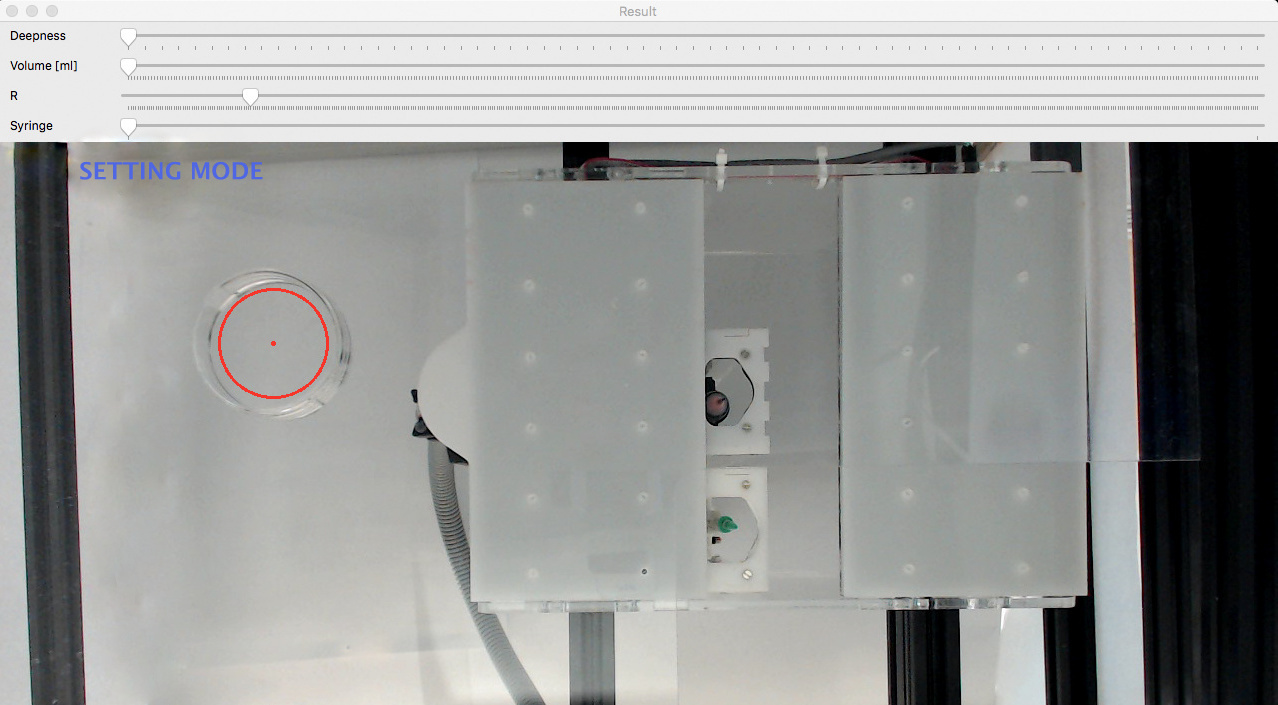
\includegraphics[width=7.5cm, height=5.5cm]{immagini/settingMOD2.jpg}}
 	\hspace{2mm}
   		{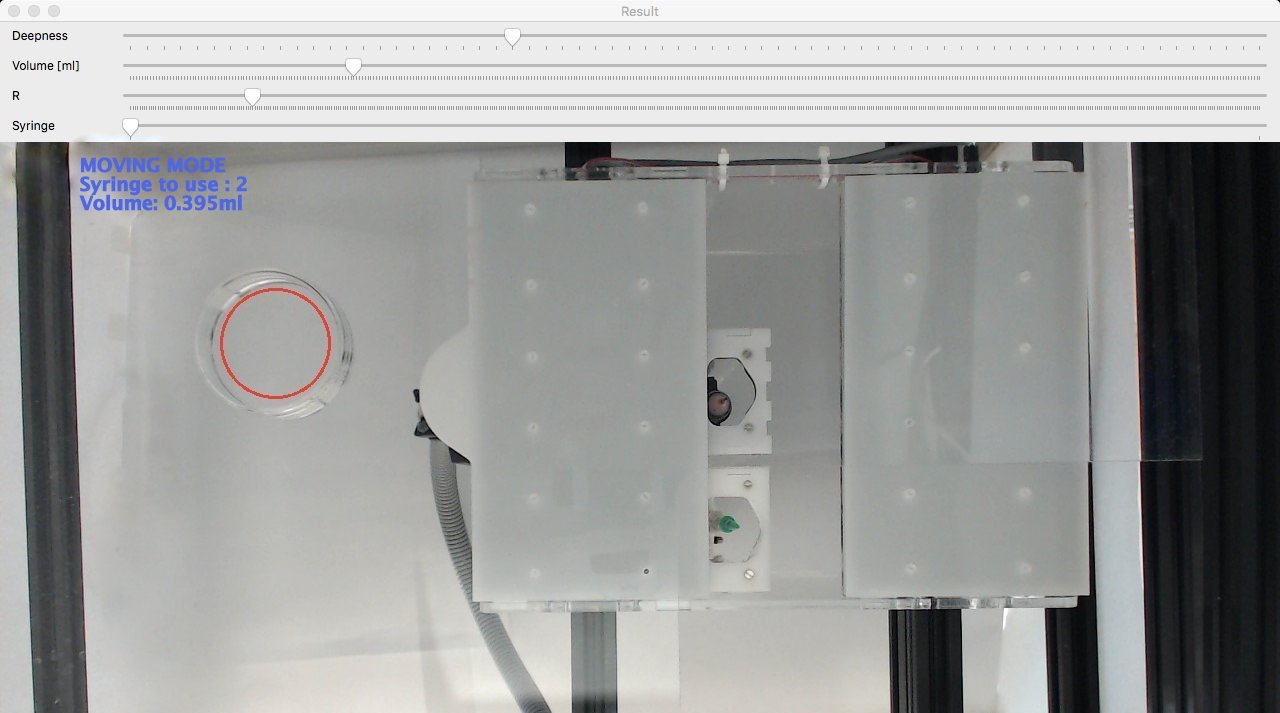
\includegraphics[width=7.5cm, height=5.5cm]{immagini/moving.jpg}}
	\caption{setting mode e moving mode}
 	\end{figure}
\\La parte superiore della finestra mostra tre barre di controllo. La prima indica la \emph{deepness} ovvero la profondità a cui il corpo della siringa deve arrivare affinché il puntale raggiunga il punto desiderato. I valori possono variare da 0 a 69, limiti di costruzione delle siringhe. Per arrivare nel punto desiderato si deve tenere in considerazione anche la lunghezza della punta della siringa per fare in modo che non vada contro il vetro. La seconda \emph{trackbar} indica il volume in $mL$ da far aspirare o rimettere alla siringa. Gli stantuffi delle siringhe utilizzate per questi esperimenti variano la loro posizione nel range da 0 a 35 perciò la \emph{trackbar} del volume è stata suddivisa in 36 porzioni, ognuna delle quali equivale a $0,14mL$. La terza \emph{trackbar} viene utilizzata nella \emph{setting mode}. Questa indica il raggio R a cui si può impostare il cerchio rosso presente in figura. Questa opzione è stata inserita per dare la possibilità di utilizzare petri dishes di diametri differenti e per annullare il rumore nel video di agenti esterni. Il cerchio rosso viene impostato per indicare l'area in cui avviene l'esperimento centrando il centro della \emph{Petri dish} ed allargando il cerchio fino ai bordi della petri stessa; questa è l'unica porzione di schermo a cui verranno applicati i filtri per la nitidezza dell'immagine, per il riconoscimento dei contorni della \emph{droplet} e per tracciarne il movimento.
La lunghezza dell'ultima \emph{trackbar} varia in base al numero di moduli siringa inseriti nella testa del robot. Con questa si può scegliere la siringa da utilizzare per una determinata azione. Quando si è nella modalità di movimento, vengono visualizzati i valori impostati nelle \emph{trackbars} in alto a sinistra nella schermata. In questa modalità l'utente può far muovere la testa del robot nei punti desiderati, spostare il corpo delle siringhe e definire i volumi di liquidi da prelevare dai pozzetti magazzino ed immettere nel sistema.  
 
\subsection{Riconoscimento della droplet}
La droplet da individuare è di colore rosso, dovuto all'aggiunta del colorante Oil Red O alla soluzione di decanolo. Tuttavia, le droplets possono essere colorate non solo con il rosso ma anche con colori scelti in base alle necessità di ogni esperimento. Per il riconoscimento di uno specifico colore si utilizza un set predefinito di tre valori che l'utente può trovare ed impostare all'interno del programma: i parametri HSV, Hue Saturation Value (tonalità, saturazione e valore). Il riconoscimento di elementi del colore impostato avviene solamente all'interno dell'area definita nella \emph{setting mode} dal cerchio rosso. 

\section{L'esperimento}
\label{sec:456}
Il protocollo seguito per i nove esperimenti prevede quattro passaggi fondamentali da eseguire nella \emph{moving mode}. 
\begin{enumerate}
\item utilizzare la siringa nella socket 2 per prelevare $50\mu L$ di decanolo dal pozzetto in posizione A
\item immettere $30\mu L$ di decanolo nella Petri Dish, contenente $9mL$ di Decanoato (Acido decanoico), in posizione C
\item  utilizzare la siringa nella socket 4 per prelevare $500\mu L$ di NaCl dal pozzetto in posizione B
\item immettere $200\mu L$ di NaCl nella Petri Dish in posizione D 
\end{enumerate}
\begin{figure}[h]
	  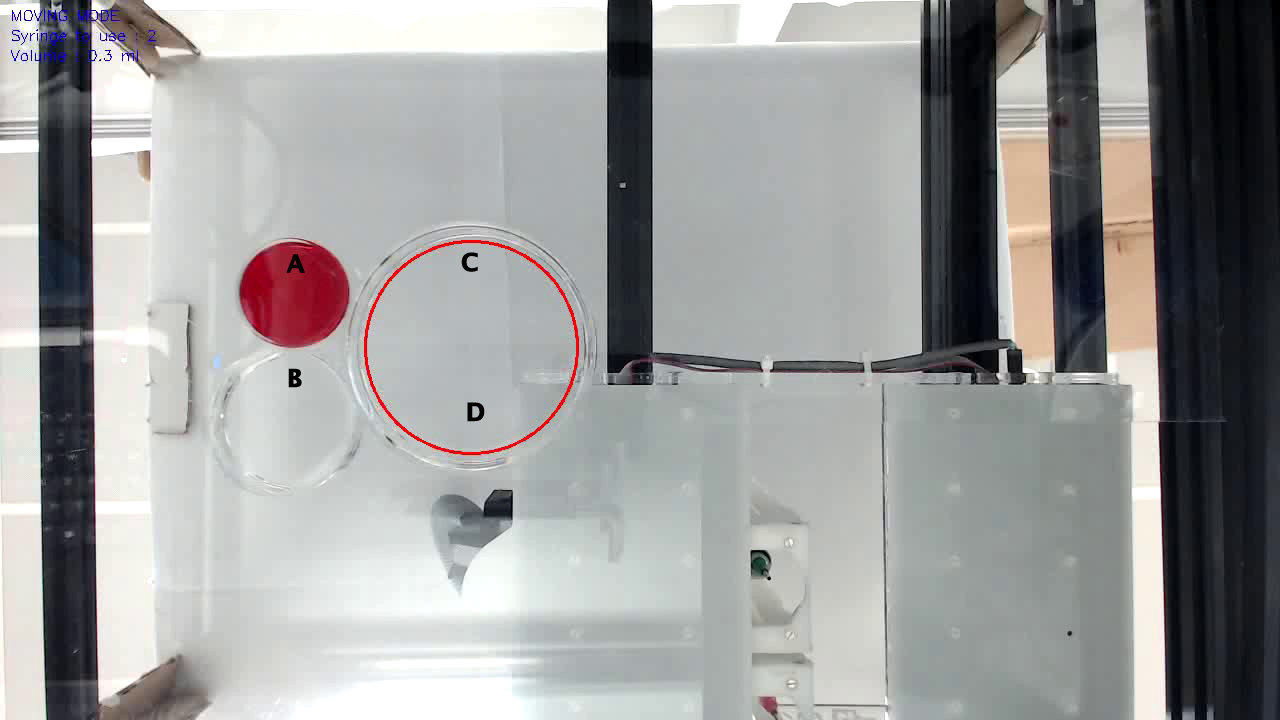
\includegraphics[scale=0.30]{immagini/exp1.jpg}
		\centering
	 \caption{experimental layout}
	\end{figure} 
La dimensione della droplet è stata definita per ottenerne una buona visibilità nella tracciabilità. 
La scelta di prelevare una quantità maggiore di liquido ci assicura l'immissione nel sistema della corretta quantità in quanto può accadere che un volume non definito venga trattenuto nel corpo o nella punta della siringa.
Le posizioni C e D all'interno della Petri sono arbitrarie e variano leggermente di esperimento in esperimento, si è cercato tuttavia, per mantenere lo spazio degli esperimenti sufficientemente uniforme, di seguire sempre lo schema proposto in figura. Questo tuttavia non è sempre stato possibile in quanto la droplet posizionata in posizione C era influenzata da moti convettivi creati dal movimento di aria attorno alla struttura del robot e dall'inserimento del puntale della siringa sulla superficie del decanoato presente nella Petri Dish. 

\subsection{Tracciabilità}
\label{sec:123}
Dopo aver posizionato la droplet di decanolo ed il sale NaCl all'interno della Petri dish, l'utente può far partire la \emph{tracking mode}. In questa modalità la testa del robot viene spostata nel punto di coordinate (0,0), in fondo a sinistra, per far in modo che non interferisca con il riconoscimento visivo. 
La droplet identificata viene circondata da un contorno verde ed indicato sulla schermata del video il colore riconosciuto. Nel momento in cui si decide di interrompere il programma, se la modalità di registrazione è attiva, appare a video il percorso eseguito dalla droplet indicante la dicitura "BEGIN" per il primo punto in cui è stata individuata, ed "END" per il punto finale di arrivo.   
\begin{figure}[h]
	\centering
   		{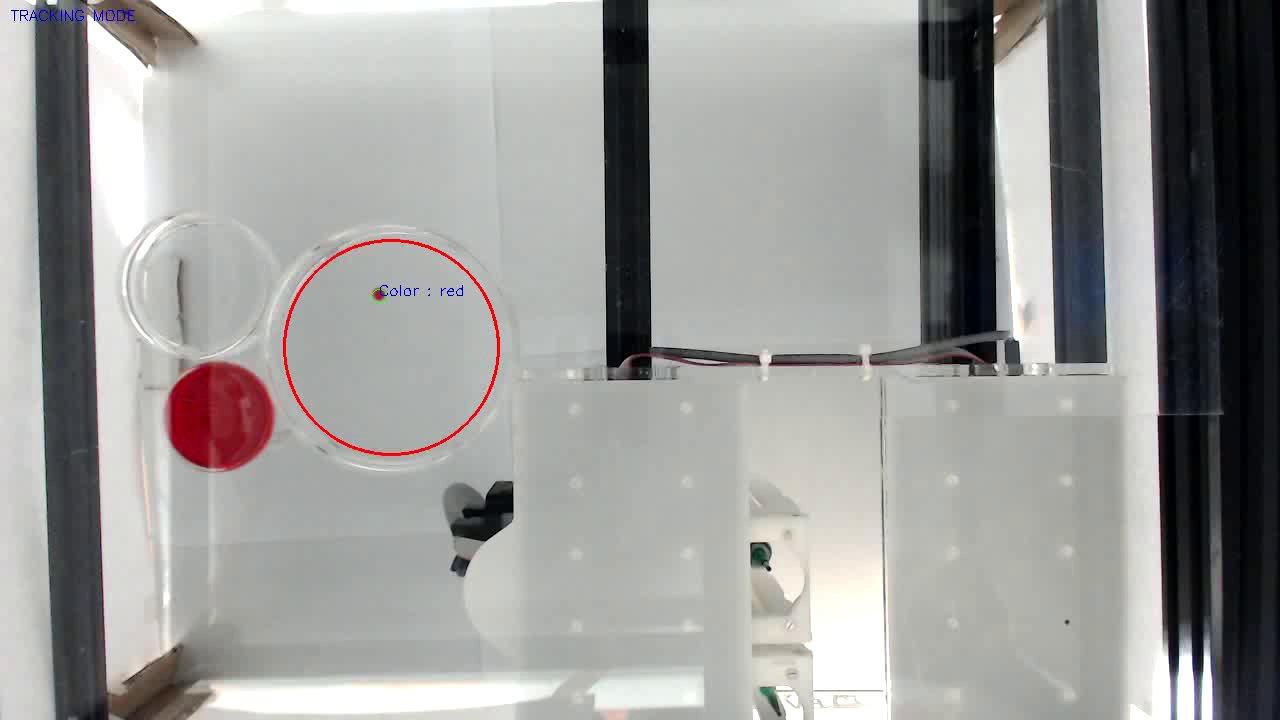
\includegraphics[width=8cm]{immagini/track.png}}
 	\hspace{2mm}   	
	{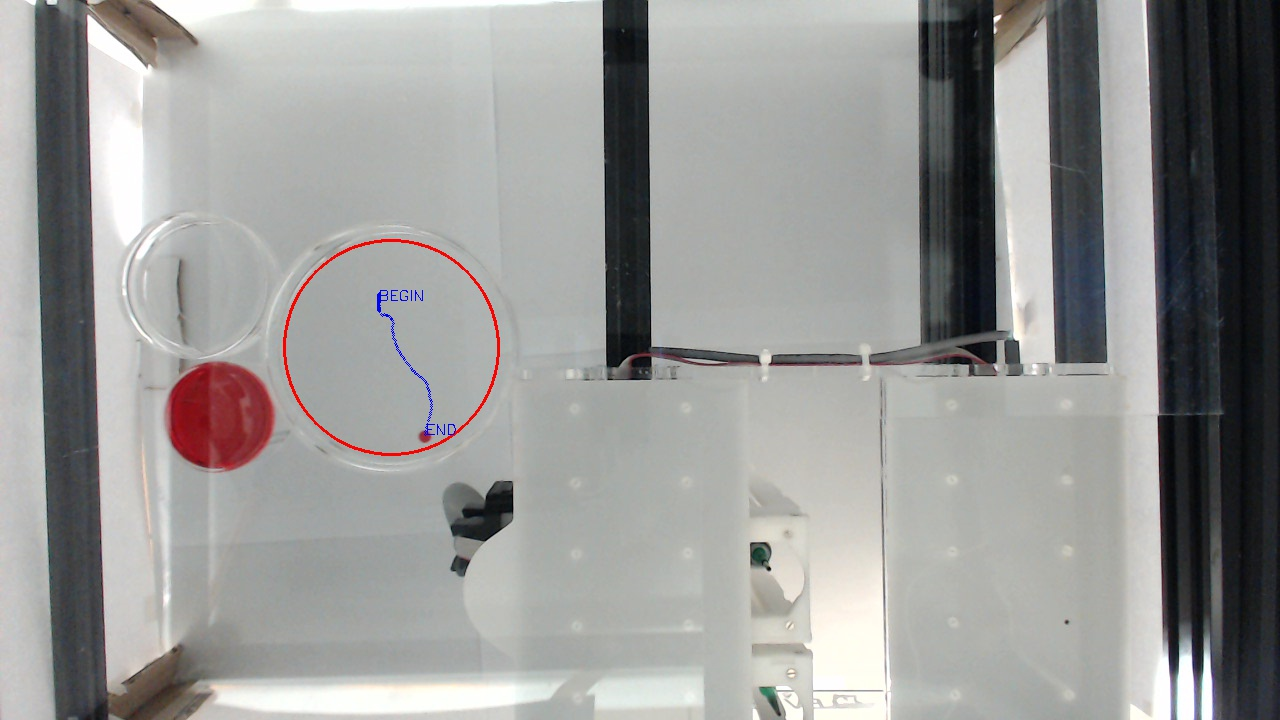
\includegraphics[width=8cm]{immagini/track_path.jpg}}
	\caption{tracking}
 	\end{figure}



\section{Dati}
Per trovare la combinazione migliore delle componenti nello spazio degli esperimenti si è applicata la funzione di adattamento per il movimento. Questa descrive la velocità media della droplet durante tutto l'esperimento ed è espressa in $1/s$. La funzione è stata applicata a due ripetizioni di ogni esperimento e la media è stata presa come valore di riferimento. La funzione è definita come:
\begin{equation*} 
\cfrac {\sqrt [ 2 ]{ { (A_{ x }-B_{ x }) }^{ 2 }+{ (A_{ y }-B_{ y }) }^{ 2 } } /\quad tempo }{ \sqrt [ 2 ]{ { (C_{ x }-B_{ x }) }^{ 2 }+{ (C_{ y }-B_{ y }) }^{ 2 }}} 
\end{equation*}
\\Dove: $A=(x,y)$ coordinate del primo punto in cui viene individuata la droplet, punto di inizio del percorso
$B=(x,y)$ coordinate del punto in cui viene inserito il sale NaCl
$C=(x,y)$ coordinate dell'ultimo punto in cui viene individuata la droplet, punto di fine percorso






























